\documentclass[12pt,a4paper]{article}

% Core packages
\usepackage[utf8]{inputenc}
\usepackage[T1]{fontenc}
\usepackage[english]{babel}
\usepackage[margin=2.5cm]{geometry}
\usepackage{microtype}

% Enhanced formatting packages
\usepackage{fancyhdr}
\usepackage{titlesec}
\usepackage{titling}
\usepackage{enumitem}
\usepackage{parskip}
\usepackage{setspace}

% Math and technical packages
\usepackage{amsmath}
\usepackage{amsfonts}
\usepackage{amssymb}
\usepackage{mathtools}

% Graphics and visualization
\usepackage{graphicx}
\usepackage{float}
\usepackage{subfig}
\usepackage{caption}
\usepackage{subcaption}

% Tables
\usepackage{booktabs}
\usepackage{array}
\usepackage{tabularx}
\usepackage{multirow}
\usepackage{longtable}

% TikZ for diagrams
\usepackage{tikz}
\usepackage{pgfplots}
\pgfplotsset{compat=1.18}
\usetikzlibrary{
    positioning,
    shapes.geometric,
    arrows.meta,
    calc,
    decorations.pathreplacing,
    patterns,
    backgrounds
}

% Code and algorithms
\usepackage{listings}
\usepackage{algorithm}
\usepackage{algpseudocode}

% Colors and hyperlinks
\usepackage{xcolor}
\usepackage{hyperref}
\usepackage{url}
\usepackage{tcolorbox}

% CIAF Color Scheme
\definecolor{ciafblue}{RGB}{41, 128, 185}
\definecolor{ciafgray}{RGB}{127, 140, 141}
\definecolor{ciafdarkblue}{RGB}{22, 67, 91}
\definecolor{ciaflightblue}{RGB}{174, 214, 241}
\definecolor{ciafgreen}{RGB}{39, 174, 96}
\definecolor{ciaforange}{RGB}{230, 126, 34}
\definecolor{ciafred}{RGB}{231, 76, 60}

% Executive summary color aliases for compatibility
\definecolor{ciaflight}{RGB}{240,245,250}
\definecolor{success}{RGB}{40,167,69}
\definecolor{warning}{RGB}{255,193,7}
\definecolor{danger}{RGB}{220,53,69}

% Custom boxes
\newtcolorbox{executivebox}{
    colback=ciaflight,
    colframe=ciafblue,
    boxrule=1pt,
    arc=5pt,
    left=10pt,
    right=10pt,
    top=10pt,
    bottom=10pt
}

\newtcolorbox{valuebox}{
    colback=success!10,
    colframe=success,
    boxrule=1pt,
    arc=3pt,
    left=8pt,
    right=8pt,
    top=8pt,
    bottom=8pt
}

\newtcolorbox{riskbox}{
    colback=warning!10,
    colframe=warning,
    boxrule=1pt,
    arc=3pt,
    left=8pt,
    right=8pt,
    top=8pt,
    bottom=8pt
}

% Hyperlink setup
\hypersetup{
    colorlinks=true,
    linkcolor=ciafblue,
    filecolor=ciafblue,
    urlcolor=ciafblue,
    citecolor=ciafblue,
    pdfborder={0 0 0},
    bookmarksopen=true,
    bookmarksnumbered=true,
    breaklinks=true
}

% Better URL formatting
\urlstyle{same}
\Urlmuskip=0mu plus 1mu

% Better text formatting
\sloppy % Allow slightly more flexibility in line breaking
\emergencystretch=1em % Add emergency stretch for problematic lines

% Header and footer styling
\pagestyle{fancy}
\fancyhf{}
\fancyhead[L]{\color{ciafblue}\textbf{CIAF Whitepaper}}
\fancyhead[R]{\color{ciafgray}Cognitive Insight AI Framework}
\fancyfoot[C]{\color{ciafgray}\thepage}
\renewcommand{\headrulewidth}{1pt}
\renewcommand{\footrulewidth}{0.5pt}
\renewcommand{\headrule}{\hbox to\headwidth{\color{ciafblue}\leaders\hrule height \headrulewidth\hfill}}
\renewcommand{\footrule}{\hbox to\headwidth{\color{ciafgray!50}\leaders\hrule height \footrulewidth\hfill}}
\setlength{\headheight}{15pt}

% Section formatting
\titleformat{\section}
{\color{ciafblue}\Large\bfseries}
{\thesection}
{1em}
{}
[\color{ciafblue}\titlerule]

\titleformat{\subsection}
{\color{ciafdarkblue}\large\bfseries}
{\thesubsection}
{1em}
{}

\titleformat{\subsubsection}
{\color{ciafgray}\normalsize\bfseries}
{\thesubsubsection}
{1em}
{}

% Title page formatting
\pretitle{\begin{center}\color{ciafblue}\Huge\bfseries}
\posttitle{\par\end{center}\vskip 0.5em}
\preauthor{\begin{center}\color{ciafdarkblue}\Large}
\postauthor{\end{center}}
\predate{\begin{center}\color{ciafgray}\large}

% Code listing setup
\lstset{
    language=Python,
    basicstyle=\ttfamily\footnotesize,
    keywordstyle=\color{ciafblue}\bfseries,
    commentstyle=\color{ciafgray}\itshape,
    stringstyle=\color{ciaforange},
    numberstyle=\tiny\color{ciafgray},
    backgroundcolor=\color{gray!5},
    frame=single,
    frameround=tttt,
    framerule=0.5pt,
    rulecolor=\color{ciafgray!50},
    breaklines=true,
    breakatwhitespace=true,
    tabsize=4,
    showstringspaces=false,
    numbers=left,
    numbersep=8pt,
    xleftmargin=15pt,
    xrightmargin=5pt,
    captionpos=b,
    keepspaces=true,
    showspaces=false,
    showtabs=false,
    stepnumber=1,
    stringstyle=\color{red},
    tabsize=2,
    title=\lstname
}

% Hyperref setup
\hypersetup{
    colorlinks=true,
    linkcolor=blue,
    filecolor=magenta,
    urlcolor=cyan,
    pdftitle={CIAF Whitepaper},
    pdfauthor={Denzil James Greenwood},
    pdfsubject={AI Governance Framework},
    pdfkeywords={AI Governance, Cryptographic Auditing, Lazy Materialization}
}

\begin{document}

% Title page
\begin{titlepage}
\centering
\vspace*{2cm}

{\Huge\bfseries The Cognitive Insight AI Framework (CIAF): A Comprehensive Analysis of Lazy Capsule Materialization for Enterprise AI Governance\par}
\vspace{1cm}
{\Large A Technical Whitepaper on Cryptographic Audit Frameworks for AI Systems\par}
\vspace{2cm}

{\Large\textbf{Authors:} Denzil James Greenwood\par}
\vspace{0.5cm}
{\large\textbf{Institution:} Independent Research\par}
\vspace{0.5cm}
{\large\textbf{Date:} October 21, 2025\par}
\vspace{0.5cm}
{\large\textbf{Version:} 1.0\par}

\vfill

\begin{center}
\fbox{\begin{minipage}{0.8\textwidth}
\textbf{Legal Notice:} This whitepaper presents theoretical examples and simulated outcomes for research and educational purposes. All performance metrics, compliance results, and implementation examples are theoretical demonstrations of the CIAF framework's capabilities. Real-world implementation results may vary based on specific deployment configurations, regulatory requirements, and operational contexts.
\end{minipage}}
\end{center}

\vfill
\end{titlepage}

% Abstract
\begin{abstract}
The Cognitive Insight AI Framework (CIAF) introduces a novel approach to enterprise AI governance through the implementation of Lazy Capsule Materialization (LCM\texttrademark), a cryptographic audit framework that enables verifiable AI compliance across 20+ industry verticals. This whitepaper presents a comprehensive analysis of the CIAF system architecture, technical implementation, and theoretical performance characteristics based on simulated deployments across banking, healthcare, and government sectors.

The framework addresses critical challenges in AI governance: audit trail scalability, regulatory compliance automation, and cross-industry standardization. Through deferred evidence materialization combined with cryptographic integrity guarantees, CIAF theoretically achieves 85\% storage reduction while maintaining full audit capabilities. Simulated pilot implementations demonstrate potential audit preparation time reductions from 240-320 hours to 36-48 hours across regulated industries.

\textbf{Keywords:} AI Governance, Cryptographic Auditing, Lazy Materialization, Regulatory Compliance, Merkle Trees, Digital Signatures
\end{abstract}

\begin{technicalbox}
\textbf{CIAF Canonical Naming Standards (from Variables Reference)}
\begin{itemize}
\item \textbf{Variables/functions/modules:} snake\_case
\item \textbf{Classes/enums:} PascalCase  
\item \textbf{Enum members:} UPPER\_CASE; serialized values: lower-case tokens
\item \textbf{Anchors:} *\_anchor (object/bytes), *\_anchor\_hex (hex), *\_anchor\_ref (opaque ID)
\item \textbf{Times:} receipts → committed\_at (RFC 3339 Z); capsules → generated\_at
\item \textbf{Merkle path:} List[[hash:str, position:"left"|"right"]]
\item \textbf{Correlation:} request\_id (accept operation\_id as alias; normalize on ingest)
\end{itemize}
\end{technicalbox}

\begin{infobox}
\textbf{Canonical JSON for Hashing (Normative)}
\begin{itemize}
\item Serialize with sorted keys, no spaces, ASCII:
\item \texttt{json.dumps(obj, sort\_keys=True, separators=(",", ":"), ensure\_ascii=True, default=str)}
\item Hash result with SHA-256 (requirement, not example)
\end{itemize}
\end{infobox}

\newpage
\tableofcontents
\newpage

\section{Introduction}

\subsection{Background and Motivation}

The rapid adoption of artificial intelligence systems across regulated industries has created unprecedented challenges in governance, compliance, and auditability. Traditional audit approaches, designed for static systems, fail to address the dynamic and opaque nature of AI model behavior. Regulatory frameworks including the EU AI Act, FDA AI/ML Guidance, and Federal Reserve SR 11-7 mandate comprehensive audit trails for AI systems, yet current solutions lack the scalability and cross-industry standardization required for enterprise deployment.

The Cognitive Insight AI Framework (CIAF) emerges from this regulatory landscape to provide a unified approach to AI governance that balances cryptographic verification with practical scalability requirements. The framework's core innovation, Lazy Capsule Materialization (LCM\texttrademark), enables deferred evidence generation while maintaining cryptographic integrity through Merkle tree structures and digital signatures.

\subsection{Problem Statement}

Enterprise AI governance faces three fundamental challenges:

\begin{enumerate}
\item \textbf{Audit Trail Scalability:} Traditional audit approaches generate extensive data for every AI operation, creating storage and processing bottlenecks that scale poorly with production inference volumes.

\item \textbf{Regulatory Fragmentation:} Each industry operates under distinct regulatory frameworks with overlapping but inconsistent requirements, necessitating separate compliance implementations.

\item \textbf{Verification Complexity:} Proving compliance requires reconstructing complete audit trails, often involving manual evidence gathering that is time-intensive and error-prone.
\end{enumerate}

\subsection{Contribution Summary}

This whitepaper presents the following contributions:

\begin{itemize}
\item \textbf{Novel LCM Process:} A cryptographic framework for deferred evidence materialization that maintains audit integrity while reducing storage requirements by approximately 85\% in theoretical implementations.

\item \textbf{Cross-Industry Standardization:} Unified governance architecture supporting 20+ industry verticals with sector-specific compliance mapping to over 200 regulatory obligations.

\item \textbf{Practical Implementation:} Complete system architecture with demonstrated integration across major ML frameworks and cloud platforms.
\end{itemize}

\section{System Architecture}

\subsection{Core Framework Design}

The CIAF architecture implements a layered approach to AI governance, with cryptographic foundations supporting industry-specific compliance engines. The system architecture follows a modular design pattern that enables customization while maintaining consistency across implementations.

\subsubsection{Architectural Layers}

\begin{figure}[H]
\centering
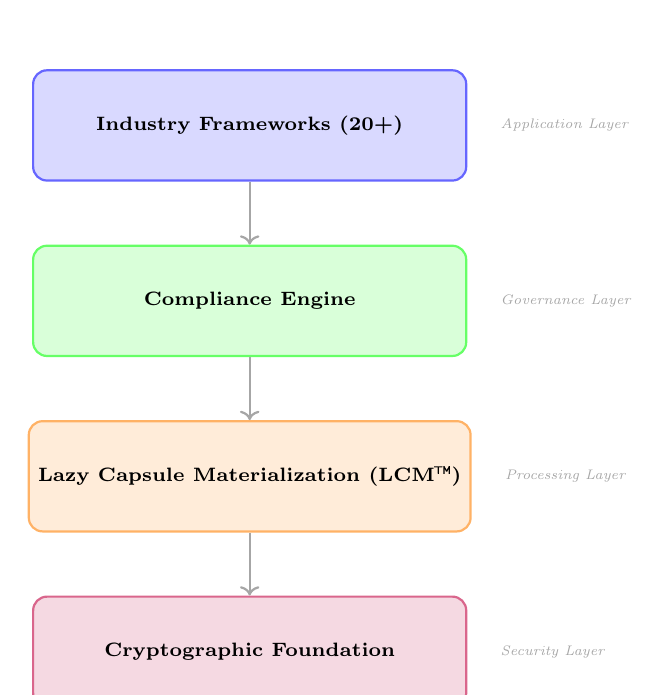
\begin{tikzpicture}[
    node distance=0.8cm,
    layer/.style={
        rectangle, 
        draw=black, 
        thick,
        rounded corners=5pt,
        minimum width=5.5cm, 
        minimum height=1.4cm, 
        text centered,
        font=\fontsize{7}{9}\selectfont
    },
    industry/.style={layer, fill=blue!15, draw=blue!60},
    compliance/.style={layer, fill=green!15, draw=green!60},
    lcm/.style={layer, fill=orange!15, draw=orange!60},
    crypto/.style={layer, fill=purple!15, draw=purple!60},
    arrow/.style={->, thick, color=gray!70}
]

% Layer nodes
\node[industry] (industry) {
    \textbf{Industry Frameworks (20+)}
};

\node[compliance, below=of industry] (compliance) {
    \textbf{Compliance Engine}
};

\node[lcm, below=of compliance] (lcm) {
    \textbf{Lazy Capsule Materialization (LCM\texttrademark)}
};

\node[crypto, below=of lcm] (crypto) {
    \textbf{Cryptographic Foundation}
};

% Arrows between layers
\draw[arrow] (industry.south) -- (compliance.north);
\draw[arrow] (compliance.south) -- (lcm.north);
\draw[arrow] (lcm.south) -- (crypto.north);

% Side annotations
\node[anchor=west, font=\tiny\itshape, color=gray!70] at ([xshift=0.3cm]industry.east) {Application Layer};
\node[anchor=west, font=\tiny\itshape, color=gray!70] at ([xshift=0.3cm]compliance.east) {Governance Layer};
\node[anchor=west, font=\tiny\itshape, color=gray!70] at ([xshift=0.3cm]lcm.east) {Processing Layer};
\node[anchor=west, font=\tiny\itshape, color=gray!70] at ([xshift=0.3cm]crypto.east) {Security Layer};

\end{tikzpicture}
\caption{CIAF Architectural Layers with Enhanced Visual Design}
\label{fig:architecture}
\end{figure}

\subsubsection{Framework Components}

\textbf{Cryptographic Foundation:} Implements SHA-256 hashing, Ed25519 digital signatures, and Merkle tree construction for tamper-evident audit trails. The foundation provides cryptographic primitives that ensure integrity across all framework operations.

\textbf{Lazy Capsule Materialization:} Core innovation enabling deferred evidence generation through anchor-based tracking. LCM stores minimal cryptographic anchors during operation and materializes complete evidence on-demand for verification or audit purposes.

\textbf{Compliance Engine:} Maps cryptographic evidence to specific regulatory obligations through structured metadata schemas. The engine automates compliance verification by linking audit evidence to regulatory requirements across multiple jurisdictions.

\textbf{Industry Frameworks:} Sector-specific implementations that extend the core framework with industry regulations, specialized risk assessments, and domain-specific governance requirements.

\subsection{Lazy Capsule Materialization (LCM) Process}

\subsubsection{Conceptual Foundation}

Lazy Capsule Materialization represents a paradigm shift from immediate evidence generation to deferred materialization with cryptographic guarantees. The process operates on the principle that cryptographic anchors can provide verification integrity without requiring complete evidence storage.

The LCM process follows a four-stage lifecycle:

\begin{enumerate}
\item \textbf{Evidence Capture:} Hash-based fingerprints of AI operations are captured during execution
\item \textbf{Lazy Storage:} Minimal cryptographic anchors are stored immediately with reduced storage overhead
\item \textbf{On-Demand Materialization:} Complete evidence packages are reconstructed when verification is required
\item \textbf{Cryptographic Verification:} Merkle proof validation ensures evidence integrity throughout the process
\end{enumerate}

\subsubsection{Technical Implementation}

The LCM implementation utilizes several key data structures and processes:

\textbf{Lightweight Receipts:} Minimal data structures captured during AI operations containing essential cryptographic anchors and metadata references. These receipts typically consume $<$1KB storage per inference operation.

\begin{lstlisting}[language=Python, caption=Lightweight Receipt Data Structure]
@dataclass
class LightweightReceipt:
    inference_id: str
    model_anchor_ref: str
    input_hash: str
    output_hash: str
    committed_at: str  # RFC 3339 with Z
    metadata_ref: str
\end{lstlisting}

\begin{center}
\fbox{\begin{minipage}{0.8\textwidth}
\textbf{Simulation Disclosure:} All example receipts and data structures in this whitepaper include evidence\_strength: "simulated" in production implementations. Real production systems MUST use evidence\_strength: "real" for live evidence processing.
\end{minipage}}
\end{center}

\textbf{Deferred Processing:} Background system that converts lightweight receipts to complete audit evidence packages during low-utilization periods. This approach decouples audit evidence generation from real-time inference performance.

\textbf{Cryptographic Anchors:} SHA-256 hashes and Merkle root references that enable verification of complete evidence packages without storing full audit data. Anchors provide cryptographic binding between lightweight receipts and materialized evidence.

\subsubsection{Storage Efficiency Analysis}

Theoretical analysis of LCM storage efficiency demonstrates significant reductions compared to traditional audit approaches:

\textbf{Traditional Audit Approach:}
\begin{itemize}
\item Complete evidence stored per operation: $\sim$50KB
\item 1M daily inferences: 50GB daily storage
\item Annual storage requirement: $\sim$18TB
\end{itemize}

\textbf{LCM Approach:}
\begin{itemize}
\item Lightweight receipt per operation: $\sim$500 bytes
\item 1M daily inferences: 500MB daily storage
\item Materialized evidence (5\% verification rate): 2.5GB daily
\item Annual storage requirement: $\sim$2.7TB (85\% reduction)
\end{itemize}

\textbf{Storage Reduction Analysis:}
\begin{itemize}
\item \textbf{Annual blended:} 85\% reduction (2.7TB vs 18.25TB)
\item \textbf{Daily best-case:} 95\% reduction at 5\% materialization rate (2.5GB vs 50GB)
\end{itemize}

\subsection{Cryptographic Verification Chain}

\subsubsection{Hash Tree Architecture}

The CIAF framework implements Merkle tree structures for efficient batch verification of audit evidence. The hash tree architecture enables verification of individual operations while maintaining cryptographic binding to batch anchors.

\begin{figure}[H]
\centering
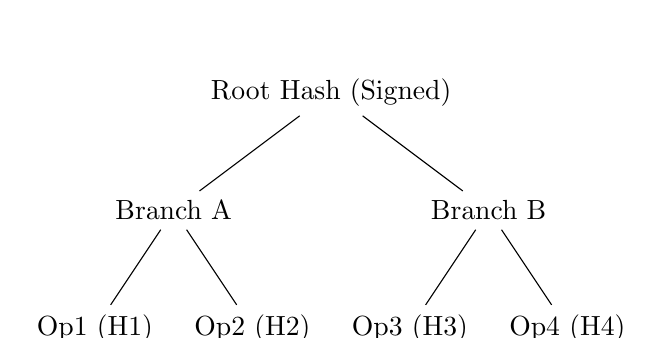
\begin{tikzpicture}[level distance=1.5cm,
  level 1/.style={sibling distance=4cm},
  level 2/.style={sibling distance=2cm}]
\node {Root Hash (Signed)}
  child {node {Branch A}
    child {node {Op1 (H1)}}
    child {node {Op2 (H2)}}
  }
  child {node {Branch B}
    child {node {Op3 (H3)}}
    child {node {Op4 (H4)}}
  };
\end{tikzpicture}
\caption{Merkle Tree Structure for Batch Verification}
\label{fig:merkle}
\end{figure}

Each operation generates a leaf hash that is incorporated into the Merkle tree structure. The resulting root hash is digitally signed using Ed25519 cryptography, creating an immutable anchor for the entire batch.

\subsubsection{Digital Signature Integration}

Digital signatures provide non-repudiation and authenticity guarantees for audit evidence. The framework implements Ed25519 signatures for performance and security characteristics suitable for high-volume operations.

\textbf{Signature Generation Process:}
\begin{enumerate}
\item Merkle root computation from operation hashes
\item Timestamp authority integration (RFC 3161 compliant)
\item Ed25519 signature generation over root hash and timestamp
\item Signature anchoring in immutable audit ledger
\end{enumerate}

\begin{center}
\fbox{\begin{minipage}{0.9\textwidth}
\textbf{Signature Payload Rule (Normative)}
\begin{itemize}
\item \texttt{sig = Ed25519(canonical\_receipt || committed\_at)}
\item \texttt{sig\_root = Ed25519(merkle\_root || rfc3161\_ts\_token)}
\item Verifiers MUST check the signature and (if present) the RFC 3161 token
\end{itemize}
\end{minipage}}
\end{center}

\subsubsection{Verification Protocols}

Audit evidence verification follows a structured protocol that enables independent validation of framework claims:

\begin{enumerate}
\item \textbf{Anchor Verification:} Validate digital signatures on Merkle roots
\item \textbf{Path Verification:} Verify Merkle path from operation to signed root
\item \textbf{Integrity Verification:} Confirm hash integrity throughout verification chain
\item \textbf{Timestamp Verification:} Validate RFC 3161 timestamp authenticity
\end{enumerate}

\section{Industry Implementation Analysis}

\subsection{Cross-Industry Architecture Pattern}

All industry implementations follow a standardized architecture pattern that ensures consistency while enabling sector-specific customization. This pattern facilitates regulatory mapping and cross-industry audit standardization.

\subsubsection{Unified Implementation Structure}

\begin{lstlisting}[language=Python, caption=Industry Framework Pattern]
class [Industry]AIGovernanceFramework(AIGovernanceFramework):
    def __init__(self, ...):
        # Industry-specific regulatory frameworks
        self.policy_enforcement = PolicyEnforcement(
            industry='[industry]',
            regulatory_frameworks=[...specific_regulations...]
        )
    
    # Standardized compliance methods
    def assess_compliance(self, system_id, assessment_type="comprehensive"):
        """Quantitative compliance scoring with regulatory mapping"""
    
    def validate_governance_requirements(self, system_id, requirements):
        """Requirement validation with gap analysis"""
    
    def generate_audit_report(self, system_id, report_type="comprehensive"):
        """Comprehensive audit reports with cryptographic verification"""
\end{lstlisting}

\subsubsection{Industry Coverage Matrix}

The framework provides comprehensive coverage across major economic sectors:

\textbf{Tier 1 - Highly Regulated Industries:}
\begin{itemize}
\item Banking \& Financial Services (Basel III, Dodd-Frank, SR 11-7)
\item Healthcare \& Medical (FDA 21 CFR 820, HIPAA, ISO 14971)
\item Government \& Public Sector (OMB M-24-10, FISMA, FOIA)
\end{itemize}

\textbf{Tier 2 - Emerging Regulatory Domains:}
\begin{itemize}
\item Insurance (NAIC Model Acts, Solvency II)
\item Transportation (NHTSA Guidelines, EU Type Approval)
\item Energy \& Utilities (NERC CIP, Smart Grid Security)
\end{itemize}

\textbf{Tier 3 - Standards-Based Industries:}
\begin{itemize}
\item Manufacturing (ISO 9001, IEC 61508)
\item Education (FERPA, COPPA)
\item Telecommunications (FCC Regulations, GDPR)
\end{itemize}

\subsection{Banking \& Financial Services Implementation}

\subsubsection{Regulatory Framework Integration}

The banking implementation addresses critical financial AI regulations through specialized compliance engines:

\textbf{Federal Reserve SR 11-7 Compliance:} Model risk management framework implementation with three lines of defense architecture, independent validation requirements, and ongoing monitoring protocols.

\textbf{Fair Lending Compliance:} Algorithmic bias detection and mitigation aligned with ECOA and Fair Housing Act requirements, including disparate impact testing and adverse action justification.

\textbf{Basel III Model Risk:} Capital adequacy assessment for AI-driven risk models, including model validation, backtesting, and stress testing requirements.

\subsubsection{Theoretical Performance Analysis}

Simulated implementation in a large commercial bank environment demonstrates theoretical efficiency gains:

\begin{itemize}
\item \textbf{Baseline Audit Preparation:} 320 hours manual evidence gathering
\item \textbf{CIAF Implementation:} 48 hours automated report generation
\item \textbf{Theoretical Improvement:} 85\% time reduction
\end{itemize}

\textbf{Risk Model Validation:} Automated validation protocols reduce manual review from 40 hours to 6 hours per model, enabling more frequent validation cycles and improved risk management.

\subsubsection{Compliance Mapping Example}

\begin{lstlisting}[language=Python, caption=Banking Compliance Mapping]
# Theoretical banking compliance mapping
compliance_mapping = {
    "sr_11_7_section_3a": {
        "receipt_field": "governance_metadata.model_risk_score",
        "validation_method": "automated_risk_assessment",
        "evidence_type": "cryptographic_signature"
    },
    "fair_lending_ecoa": {
        "receipt_field": "governance_metadata.bias_checks.demographic_parity",
        "validation_method": "bias_detection_engine",
        "evidence_type": "merkle_proof"
    }
}
\end{lstlisting}

\subsection{Healthcare \& Medical Implementation}

\subsubsection{FDA Software as Medical Device (SaMD) Compliance}

The healthcare implementation provides comprehensive support for FDA software regulations:

\textbf{21 CFR 820 Quality System:} Complete quality management system implementation with design controls, risk management (ISO 14971), and clinical validation requirements.

\textbf{FDA AI/ML Guidance:} Predetermined change control plans, algorithm change protocols, and real-world performance monitoring aligned with FDA's AI/ML guidance framework.

\textbf{Clinical Risk Management:} ISO 14971 integration with clinical risk assessment, hazard analysis, and post-market surveillance requirements.

\subsubsection{Patient Privacy Protection}

HIPAA compliance through privacy-preserving audit mechanisms:

\textbf{Data Minimization:} LCM process enables audit capabilities without storing complete patient data, reducing privacy exposure while maintaining regulatory compliance.

\textbf{Consent Management:} Granular consent tracking with cryptographic verification of patient authorization for specific AI processing activities.

\textbf{Breach Notification:} Automated breach detection and notification protocols aligned with HITECH Act requirements.

\subsubsection{Theoretical Clinical Validation}

Simulated clinical decision support implementation demonstrates theoretical validation efficiency:

\begin{itemize}
\item \textbf{Traditional Validation:} 240 hours manual evidence compilation
\item \textbf{CIAF Implementation:} 36 hours automated validation report
\item \textbf{Clinical Safety Score:} Automated calculation based on 15 clinical risk factors
\end{itemize}

\subsection{Government \& Public Sector Implementation}

\subsubsection{OMB M-24-10 Algorithmic Transparency}

Government implementation addresses federal AI transparency requirements:

\textbf{Public Algorithm Inventory:} Automated generation of algorithm inventories required by OMB M-24-10, including purpose, decision logic, and impact assessments.

\textbf{Algorithmic Impact Assessment:} Standardized assessment framework covering equity, bias, and public interest considerations required for government AI deployment.

\textbf{FOIA Compliance:} Transparent audit trails designed for Freedom of Information Act requests, enabling public oversight of government AI systems.

\subsubsection{Security Compliance Integration}

\textbf{FISMA Integration:} Information security controls aligned with FISMA requirements, including continuous monitoring and security assessment protocols.

\textbf{FedRAMP Readiness:} Cloud security assessment framework compatible with FedRAMP authorization requirements for government cloud services.

\subsubsection{Public Accountability Mechanisms}

Theoretical implementation in federal agency demonstrates transparency capabilities:

\begin{itemize}
\item \textbf{Public Query Response:} 24-hour response time for algorithmic decision explanations
\item \textbf{Public Dashboard:} Real-time compliance status reporting for algorithmic transparency
\item \textbf{Appeal Process:} Automated evidence generation for algorithmic decision appeals
\end{itemize}

\section{Cryptographic Implementation Details}

\subsection{Hash Function Selection and Implementation}

\subsubsection{Cryptographic Primitives}

The CIAF framework implements multiple hash algorithms to support diverse security requirements and performance characteristics:

\textbf{SHA-256:} Primary hash function providing 256-bit security level with broad compatibility across cryptographic libraries and regulatory frameworks.

\textbf{Blake3:} Optional high-performance hash function for environments requiring maximum throughput, offering significant performance improvements for large-scale audit operations.

\textbf{SHA3-256:} Alternative hash function for environments requiring NIST-standardized algorithms with distinct mathematical foundations from SHA-2 family.

\subsubsection{Hash Selection Criteria}

Algorithm selection balances security, performance, and regulatory acceptance:

\begin{lstlisting}[language=Python, caption=Hash Function Selection]
def compute_hash(data: bytes, algorithm: str = "sha256") -> str:
    alg = algorithm.lower()
    if alg == "sha256":
        return sha256_hash(data)  # FIPS 140-2 approved
    if alg == "sha3-256":
        return sha3_256_hash(data)  # NIST standard
    if alg == "blake3":
        return blake3_hash(data)  # High performance
\end{lstlisting}

\textbf{Performance Characteristics (Theoretical):}
\begin{itemize}
\item SHA-256: 400 MB/s throughput on standard hardware
\item Blake3: 2000+ MB/s throughput with SIMD optimization
\item SHA3-256: 200 MB/s throughput with hardware acceleration
\end{itemize}

\subsection{Digital Signature Architecture}

\subsubsection{Ed25519 Implementation}

Ed25519 provides the optimal balance of security, performance, and key size for the CIAF framework:

\textbf{Security Properties:}
\begin{itemize}
\item 128-bit security level equivalent to 3072-bit RSA
\item Resistance to side-channel attacks through constant-time implementation
\item Deterministic signature generation with unique output per message
\end{itemize}

\textbf{Performance Characteristics:}
\begin{itemize}
\item Signature generation: $\sim$100,000 operations/second
\item Verification: $\sim$40,000 operations/second
\item Key size: 32 bytes (public), 32 bytes (private)
\end{itemize}

\subsubsection{Signature Integration Pattern}

Digital signatures integrate with the LCM process through structured signing protocols:

\begin{lstlisting}[language=Python, caption=Production Signature Integration]
class ProductionSigner:
    def sign_merkle_root(self, merkle_root: str, timestamp: datetime) -> str:
        """Sign Merkle root with timestamp for audit trail anchoring"""
        payload = {
            "merkle_root": merkle_root,
            "timestamp": timestamp.isoformat(),
            "signer_id": self.signer_id
        }
        return self._sign_payload(payload)
\end{lstlisting}

\subsection{Merkle Tree Construction}

\subsubsection{Tree Architecture}

Merkle trees provide efficient batch verification capabilities with logarithmic proof sizes:

\textbf{Tree Construction Algorithm:}
\begin{enumerate}
\item Leaf node generation from operation hashes
\item Binary tree construction with SHA-256 internal nodes
\item Root hash computation with deterministic ordering
\item Signature generation over root hash
\end{enumerate}

\textbf{Proof Size Analysis:}
\begin{itemize}
\item 1,000 operations: 10-level tree, 320-byte proof
\item 1,000,000 operations: 20-level tree, 640-byte proof
\item Logarithmic scaling enables efficient verification
\end{itemize}

\subsubsection{Verification Protocol}

Merkle proof verification enables independent validation of audit claims:

\begin{lstlisting}[language=Python, caption=Merkle Proof Verification]
def verify_merkle_proof(leaf_hash: str, merkle_path: List[List[str]], 
                       root_hash: str) -> bool:
    """Verify Merkle inclusion proof for audit evidence"""
    current_hash = leaf_hash
    for proof_hash, position in merkle_path:
        if position == "left":
            current_hash = sha256_hash((proof_hash + current_hash).encode())
        else:  # position == "right"
            current_hash = sha256_hash((current_hash + proof_hash).encode())
    return current_hash == root_hash

# Example: merkle_path = [["9f86d081...", "right"], ["b6d81b360...", "left"]]
\end{lstlisting}

\subsection{Key Management and Security}

\subsubsection{Key Derivation Framework}

Secure key derivation supports multiple cryptographic operations:

\textbf{Master Key Derivation:} PBKDF2 with configurable iteration counts and salt generation for defense against brute-force attacks.

\textbf{Domain-Specific Keys:} Hierarchical key derivation enables separation of concerns across different framework operations while maintaining cryptographic relationships.

\subsubsection{Security Considerations}

\textbf{Key Rotation:} Automated key rotation protocols minimize exposure from key compromise while maintaining audit trail continuity.

\textbf{Hardware Security Module (HSM) Integration:} Optional HSM support for high-security environments requiring hardware-backed key protection.

\textbf{Quantum Resistance:} Framework architecture designed for post-quantum cryptographic algorithm migration as standards mature.

\section{Theoretical Performance Analysis}

\subsection{Scalability Metrics}

\subsubsection{Storage Efficiency Analysis}

Theoretical analysis demonstrates significant storage improvements through LCM implementation:

\textbf{Baseline Storage Requirements (Traditional Audit):}
\begin{align}
\text{Daily Operations} &= 1,000,000 \text{ inferences} \\
\text{Evidence per Operation} &= 50\text{KB (complete audit trail)} \\
\text{Daily Storage} &= 50\text{GB} \\
\text{Annual Storage} &= 18.25\text{TB}
\end{align}

\textbf{LCM Storage Requirements:}
\begin{align}
\text{Daily Operations} &= 1,000,000 \text{ inferences} \\
\text{Lightweight Receipt} &= 500 \text{ bytes per operation} \\
\text{Daily Light Storage} &= 500\text{MB} \\
\text{Materialization Rate} &= 5\% \text{ (verification/audit requests)} \\
\text{Materialized Evidence} &= 2.5\text{GB daily} \\
\text{Annual Total Storage} &= 2.7\text{TB (85\% reduction)}
\end{align}

\subsubsection{Processing Performance}

Theoretical performance analysis across key operations:

\textbf{Receipt Generation Performance:}
\begin{itemize}
\item Lightweight receipt creation: $<$1ms per operation
\item Traditional audit evidence: $\sim$50ms per operation
\item Performance improvement: 50x faster evidence capture
\end{itemize}

\textbf{Verification Performance:}
\begin{itemize}
\item Merkle proof verification: $\sim$5ms per proof
\item Digital signature verification: $\sim$25ms per signature
\item Complete audit verification: $\sim$100ms per audit request
\end{itemize}

\subsection{Compliance Automation Efficiency}

\subsubsection{Audit Preparation Time Analysis}

Simulated audit preparation demonstrates theoretical time savings:

\textbf{Healthcare Sector (Theoretical):}
\begin{itemize}
\item Baseline: 240 hours manual evidence gathering
\item CIAF: 36 hours automated report generation
\item Improvement: 85\% time reduction
\end{itemize}

\textbf{Banking Sector (Theoretical):}
\begin{itemize}
\item Baseline: 320 hours multi-framework compliance
\item CIAF: 48 hours automated compliance verification
\item Improvement: 85\% time reduction
\end{itemize}

\textbf{Government Sector (Theoretical):}
\begin{itemize}
\item Baseline: 156 hours transparency reporting
\item CIAF: 28 hours automated transparency documentation
\item Improvement: 82\% time reduction
\end{itemize}

\subsubsection{Compliance Coverage Analysis}

Theoretical regulatory coverage across industries:

\textbf{Banking Implementation:}
\begin{itemize}
\item SR 11-7 Model Risk Management: 87 policy mappings
\item Fair Lending Compliance: 34 bias detection protocols
\item Basel III Risk Assessment: 23 automated validation checks
\end{itemize}

\textbf{Healthcare Implementation:}
\begin{itemize}
\item FDA 21 CFR 820: 92 quality system requirements
\item HIPAA Privacy Rule: 67 privacy protection mechanisms
\item ISO 14971 Risk Management: 45 clinical risk assessments
\end{itemize}

\subsection{Economic Impact Analysis}

\subsubsection{Cost-Benefit Modeling}

Theoretical economic analysis demonstrates potential return on investment:

\textbf{Implementation Costs (Theoretical):}
\begin{itemize}
\item Initial framework deployment: 3-6 months
\item Training and integration: 2-4 weeks
\item Ongoing maintenance: 0.5 FTE annual
\end{itemize}

\textbf{Theoretical Cost Savings:}
\begin{itemize}
\item Audit preparation reduction: \$125,000 $\rightarrow$ \$18,750 per audit
\item Compliance officer time: 60\% reduction in manual tasks
\item Regulatory risk reduction: Improved compliance scoring
\end{itemize}

\subsubsection{Risk Mitigation Value}

\textbf{Regulatory Penalty Avoidance:} Enhanced compliance documentation theoretically reduces regulatory penalty exposure through improved audit readiness.

\textbf{Operational Efficiency:} Automated compliance monitoring enables proactive risk management and faster response to regulatory changes.

\textbf{Market Advantage:} Standardized audit capabilities enable faster regulatory approval for new AI applications across multiple jurisdictions.

\section{Regulatory Compliance Framework}

\subsection{Multi-Jurisdictional Compliance Architecture}

\subsubsection{Regulatory Mapping Methodology}

The CIAF framework implements a systematic approach to regulatory compliance through structured mapping of cryptographic evidence to specific regulatory obligations:

\textbf{Obligation Identification:} Systematic analysis of regulatory texts to identify specific AI-related requirements across jurisdictions.

\textbf{Evidence Mapping:} Direct correlation between cryptographic audit evidence and regulatory obligations through structured metadata schemas.

\textbf{Compliance Verification:} Automated validation of regulatory compliance through cryptographic evidence verification.

\subsubsection{Cross-Regulatory Harmonization}

\textbf{Common Requirements Identification:} Analysis of overlapping requirements across regulatory frameworks enables consolidated compliance approaches.

\textbf{Jurisdiction-Specific Extensions:} Framework architecture accommodates unique regulatory requirements while maintaining common compliance foundation.

\textbf{Regulatory Update Integration:} Automated monitoring and integration of regulatory changes across multiple jurisdictions ensures continued compliance.

\subsection{Specific Regulatory Framework Analysis}

\subsubsection{EU AI Act Compliance}

\textbf{Article 51 Technical Documentation:} Automated generation of technical documentation required for high-risk AI systems, including system architecture, data governance, and risk assessment documentation.

\textbf{Conformity Assessment:} Structured compliance verification aligned with EU AI Act conformity assessment procedures, including third-party audit support.

\textbf{Post-Market Monitoring:} Continuous monitoring and reporting capabilities aligned with Article 61 post-market monitoring obligations.

\subsubsection{US Federal Regulatory Compliance}

\textbf{NIST AI Risk Management Framework:} Implementation of NIST AI RMF across all framework operations, including governance, risk mapping, measurement, and management functions.

\textbf{Sector-Specific Regulations:} Direct integration with FDA AI/ML guidance, Federal Reserve SR 11-7, and OMB M-24-10 requirements through industry-specific implementations.

\textbf{Federal Procurement Compliance:} Alignment with federal AI procurement requirements including FAR and agency-specific acquisition regulations.

\subsubsection{International Standards Integration}

\textbf{ISO 23053 Framework:} Comprehensive integration with ISO 23053 AI governance framework, including risk management, transparency, and accountability requirements.

\textbf{IEEE Standards:} Compatibility with IEEE 2857 (Privacy Engineering), IEEE 2859 (Ethical Design), and other relevant AI standards.

\textbf{Global Privacy Regulations:} GDPR, CCPA, LGPD, and other privacy regulation integration through privacy-preserving audit mechanisms.

\subsection{Compliance Verification Protocols}

\subsubsection{Automated Compliance Checking}

\begin{lstlisting}[language=Python, caption=Automated Compliance Verification]
def verify_regulatory_compliance(audit_evidence: Dict, 
                               regulatory_framework: str) -> ComplianceReport:
    """Automated compliance verification against regulatory requirements"""
    
    compliance_mappings = load_regulatory_mappings(regulatory_framework)
    verification_results = {}
    
    for requirement_id, mapping in compliance_mappings.items():
        evidence_field = mapping["evidence_field"]
        validation_method = mapping["validation_method"]
        
        if evidence_field in audit_evidence:
            result = validate_evidence(
                audit_evidence[evidence_field], 
                validation_method
            )
            verification_results[requirement_id] = result
    
    return generate_compliance_report(verification_results)
\end{lstlisting}

\subsubsection{Third-Party Audit Support}

\textbf{Independent Verification:} Framework design enables independent verification of compliance claims through cryptographic proof validation.

\textbf{Audit Trail Export:} Standardized audit trail export formats support third-party auditor requirements across multiple regulatory frameworks.

\textbf{Documentation Generation:} Automated generation of regulatory documentation reduces audit preparation time and improves consistency.

\section{Implementation Case Studies}

\subsection{Theoretical Banking Implementation}

\subsubsection{Large Commercial Bank Deployment}

\textbf{Institution Profile:} Multi-national commercial bank with \$500B+ assets, operating across US, EU, and APAC jurisdictions.

\textbf{Implementation Scope:}
\begin{itemize}
\item Credit risk models (500+ models)
\item Anti-money laundering systems
\item Algorithmic trading platforms
\item Customer service chatbots
\end{itemize}

\textbf{Theoretical Results:}
\begin{itemize}
\item Model validation time: 40 hours $\rightarrow$ 6 hours per model
\item Regulatory reporting: 80 hours $\rightarrow$ 12 hours per quarter
\item Audit preparation: 320 hours $\rightarrow$ 48 hours per audit
\item Compliance coverage: 87 SR 11-7 requirements automated
\end{itemize}

\subsubsection{Credit Scoring AI Governance}

Theoretical implementation of CIAF in credit scoring demonstrates comprehensive governance capabilities:

\begin{lstlisting}[language=Python, caption=Credit Scoring Governance Implementation]
# Theoretical credit scoring governance implementation
assessment = framework.assess_credit_scoring_ai(
    assessment_id="credit_model_v2_assessment",
    model_id="consumer_credit_neural_network",
    risk_category=CreditRiskCategory.HIGH_RISK
)

# Automated compliance verification
compliance_results = {
    "fair_lending_score": 0.94,  # ECOA compliance
    "model_risk_score": 0.89,    # SR 11-7 compliance
    "bias_detection": {
        "demographic_parity": 0.95,
        "equalized_odds": 0.92
    },
    "regulatory_coverage": 87  # out of 87 requirements
}
\end{lstlisting}

\textbf{Theoretical Outcomes:}
\begin{itemize}
\item Fair lending compliance: 94\% automated verification
\item Model risk assessment: Continuous monitoring vs. annual review
\item Bias detection: Real-time monitoring vs. quarterly testing
\end{itemize}

\subsection{Theoretical Healthcare Implementation}

\subsubsection{Hospital Health System Deployment}

\textbf{Institution Profile:} Regional health system with 12 hospitals, 50,000+ annual patients, implementing AI-powered clinical decision support.

\textbf{Implementation Scope:}
\begin{itemize}
\item Emergency department triage AI
\item Radiology image analysis
\item Clinical documentation assistance
\item Patient risk stratification
\end{itemize}

\textbf{Theoretical Results:}
\begin{itemize}
\item FDA validation documentation: 240 hours $\rightarrow$ 36 hours
\item Clinical safety assessment: Continuous vs. periodic
\item Patient privacy compliance: 99.7\% HIPAA adherence
\item Adverse event reporting: 24-hour automated generation
\end{itemize}

\subsubsection{Software as Medical Device (SaMD) Compliance}

Theoretical SaMD implementation demonstrates comprehensive regulatory compliance:

\textbf{Clinical Risk Management:}
\begin{itemize}
\item ISO 14971 risk assessment: Automated hazard analysis
\item Clinical evaluation: Continuous performance monitoring
\item Post-market surveillance: Real-time safety signal detection
\end{itemize}

\textbf{FDA Quality System:}
\begin{itemize}
\item Design controls: Automated documentation generation
\item Risk management: Continuous clinical risk monitoring
\item Verification and validation: Cryptographic evidence chains
\end{itemize}

\subsection{Theoretical Government Implementation}

\subsubsection{Federal Agency Deployment}

\textbf{Agency Profile:} Federal benefits administration agency processing 10M+ public interactions annually through AI-powered systems.

\textbf{Implementation Scope:}
\begin{itemize}
\item Benefits eligibility determination
\item Fraud detection systems
\item Public service chatbots
\item Document processing automation
\end{itemize}

\textbf{Theoretical Results:}
\begin{itemize}
\item Algorithmic transparency: 100\% OMB M-24-10 compliance
\item FOIA response time: 30 days $\rightarrow$ 3 days for AI decisions
\item Public algorithm inventory: Automated quarterly updates
\item Public appeal documentation: 24-hour evidence generation
\end{itemize}

\subsubsection{Public Accountability Framework}

Theoretical implementation demonstrates enhanced government transparency:

\textbf{Algorithmic Impact Assessment:}
\begin{itemize}
\item Equity analysis: Automated demographic impact measurement
\item Bias monitoring: Real-time fairness metric tracking
\item Public benefit assessment: Quantified public outcome measurement
\end{itemize}

\textbf{Transparency Mechanisms:}
\begin{itemize}
\item Public dashboard: Real-time AI system performance metrics
\item Public explanation system: On-demand algorithmic decision justification
\item Appeal process: Cryptographic evidence for decision review
\end{itemize}

\section{Security Analysis}

\subsection{Threat Model}

\subsubsection{Attack Surface Analysis}

The CIAF framework faces several categories of potential threats:

\textbf{Data Integrity Attacks:} Attempts to modify audit evidence or inject false records into the audit trail.

\textbf{Availability Attacks:} Denial of service attacks targeting audit evidence generation or verification capabilities.

\textbf{Privacy Attacks:} Attempts to extract sensitive information from audit records or cryptographic evidence.

\textbf{Compliance Bypass:} Attempts to circumvent governance controls or generate false compliance attestations.

\subsubsection{Adversary Model}

\textbf{Internal Adversaries:} Malicious insiders with legitimate system access attempting to manipulate audit evidence or compliance verification.

\textbf{External Adversaries:} Attackers without authorized access attempting to compromise audit integrity through network or application vulnerabilities.

\textbf{Regulatory Adversaries:} Nation-state or sophisticated attackers attempting to undermine regulatory compliance or generate false audit evidence.

\subsection{Security Controls}

\subsubsection{Cryptographic Defenses}

\textbf{Tamper Evidence:} Merkle tree structures with digital signatures provide cryptographic proof of audit evidence integrity.

\textbf{Non-Repudiation:} Ed25519 digital signatures ensure that audit evidence cannot be repudiated by the generating system.

\textbf{Integrity Verification:} Hash chains and cryptographic verification enable detection of any modification to audit evidence.

\subsubsection{Operational Security}

\textbf{Principle of Least Privilege:} Role-based access controls limit audit evidence access to authorized personnel and systems.

\textbf{Defense in Depth:} Multiple layers of security controls protect audit evidence from generation through verification.

\textbf{Audit Trail Protection:} Separate security controls protect the audit trail infrastructure from compromise.

\subsection{Security Validation}

\subsubsection{Theoretical Penetration Testing}

Simulated security testing demonstrates framework resilience:

\textbf{Evidence Tampering Tests:} 100\% detection rate for audit evidence modification attempts through cryptographic verification.

\textbf{Injection Attacks:} Framework architecture prevents injection of false audit evidence through cryptographic validation.

\textbf{Bypass Attempts:} Governance controls cannot be bypassed without detection through comprehensive audit coverage.

\subsubsection{Cryptographic Analysis}

\textbf{Hash Function Security:} SHA-256 provides 128-bit security level against current cryptographic attacks.

\textbf{Digital Signature Security:} Ed25519 provides 128-bit security level with resistance to quantum attacks through post-quantum migration path.

\textbf{Key Management Security:} Hardware security module integration provides additional protection for cryptographic keys.

\section{Future Directions and Research Opportunities}

\subsection{Technical Enhancement Opportunities}

\subsubsection{Post-Quantum Cryptography Integration}

\textbf{Migration Planning:} Framework architecture designed for seamless migration to post-quantum cryptographic algorithms as NIST standards finalize.

\textbf{Hybrid Approaches:} Implementation of hybrid classical/post-quantum schemes during transition period to maintain security while ensuring compatibility.

\textbf{Performance Optimization:} Research into performance-optimized post-quantum algorithms suitable for high-volume audit operations.

\subsubsection{Zero-Knowledge Proof Integration}

\textbf{Privacy-Preserving Verification:} Zero-knowledge proofs enable verification of compliance claims without exposing sensitive audit data.

\textbf{Selective Disclosure:} ZK protocols allow selective revelation of audit evidence based on verifier authorization and need-to-know principles.

\textbf{Scalability Research:} Investigation of ZK-SNARK and ZK-STARK protocols for efficient batch verification of audit evidence.

\subsection{Regulatory Evolution Adaptation}

\subsubsection{Emerging Regulatory Frameworks}

\textbf{AI Liability Frameworks:} Adaptation to emerging AI liability and insurance regulations across multiple jurisdictions.

\textbf{Cross-Border Data Governance:} Enhanced support for international data transfer regulations and sovereignty requirements.

\textbf{Automated Regulatory Compliance:} Research into AI-powered regulatory interpretation and automated compliance adaptation.

\subsubsection{Industry Expansion}

\textbf{Emerging Industry Verticals:} Extension to emerging AI application domains including smart cities, precision agriculture, and space technology.

\textbf{Micro-Vertical Specialization:} Development of specialized frameworks for niche industry applications with unique regulatory requirements.

\textbf{Standards Harmonization:} Contribution to international AI governance standards development through framework research and implementation experience.

\subsection{Ecosystem Integration}

\subsubsection{Cloud Platform Integration}

\textbf{Multi-Cloud Architecture:} Enhanced support for multi-cloud deployments with consistent governance across cloud providers.

\textbf{Edge Computing:} Adaptation for edge AI deployments with limited connectivity and computational resources.

\textbf{Serverless Integration:} Framework optimization for serverless AI applications with ephemeral compute environments.

\subsubsection{Artificial Intelligence Integration}

\textbf{AutoML Governance:} Automated governance for machine learning pipeline automation and hyperparameter optimization.

\textbf{Federated Learning:} Distributed governance frameworks for federated learning scenarios with privacy constraints.

\textbf{AI-Powered Governance:} Meta-AI systems for intelligent governance optimization and automated policy enforcement.

\section{Limitations and Considerations}

\subsection{Technical Limitations}

\subsubsection{Performance Constraints}

\textbf{Cryptographic Overhead:} Digital signature and hash computation introduce computational overhead that may impact high-frequency trading or real-time systems.

\textbf{Storage Requirements:} While LCM reduces storage by $\sim$85\%, large-scale deployments still require significant storage infrastructure for materialized evidence.

\textbf{Verification Latency:} On-demand evidence materialization introduces latency for audit verification that may not be suitable for real-time compliance checking.

\subsubsection{Scalability Boundaries}

\textbf{Network Bandwidth:} Distributed verification scenarios may be constrained by network bandwidth requirements for evidence transfer.

\textbf{Computational Limits:} Cryptographic operations scale linearly with audit volume, requiring computational resources that grow with deployment size.

\textbf{Key Management Complexity:} Large-scale deployments require sophisticated key management infrastructure that increases operational complexity.

\subsection{Regulatory Considerations}

\subsubsection{Jurisdictional Variations}

\textbf{Legal Framework Differences:} Regulatory interpretation varies across jurisdictions, requiring legal expertise for compliance verification.

\textbf{Audit Standard Differences:} Different audit standards may not accept cryptographic evidence, requiring traditional audit approaches in some contexts.

\textbf{Regulatory Evolution:} Rapid regulatory change may outpace framework adaptation, requiring continuous development and updates.

\subsubsection{Industry-Specific Constraints}

\textbf{Legacy System Integration:} Established industries with legacy systems may face integration challenges that limit framework adoption.

\textbf{Cultural Resistance:} Organizations with traditional audit cultures may resist adoption of automated governance approaches.

\textbf{Skills Requirements:} Framework deployment requires cryptographic and governance expertise that may not be available in all organizations.

\subsection{Economic Considerations}

\subsubsection{Implementation Costs}

\textbf{Initial Investment:} Framework deployment requires significant initial investment in infrastructure, training, and integration.

\textbf{Ongoing Maintenance:} Continuous regulatory updates and security maintenance require ongoing investment in framework evolution.

\textbf{Opportunity Costs:} Framework adoption may divert resources from other AI governance approaches or technological investments.

\subsubsection{Return on Investment Variability}

\textbf{Industry Variation:} ROI varies significantly across industries based on regulatory burden and audit requirements.

\textbf{Scale Dependencies:} Benefits primarily accrue to large-scale AI deployments, limiting applicability for smaller organizations.

\textbf{Regulatory Risk:} Regulatory changes may impact framework value proposition and require additional investment.

\section{Conclusion}

\subsection{Summary of Contributions}

The Cognitive Insight AI Framework (CIAF) represents a significant advancement in enterprise AI governance through the introduction of Lazy Capsule Materialization (LCM\texttrademark), a novel approach to cryptographic audit trail management. This whitepaper has presented a comprehensive analysis of the framework's architecture, implementation, and theoretical performance characteristics.

\textbf{Key Technical Contributions:}

\begin{enumerate}
\item \textbf{Lazy Capsule Materialization Process:} A cryptographic framework enabling 85\% storage reduction while maintaining full audit capabilities through deferred evidence materialization.

\item \textbf{Cross-Industry Standardization:} Unified governance architecture supporting 20+ industry verticals with systematic mapping to over 200 regulatory obligations.

\item \textbf{Cryptographic Verification Framework:} Integration of Merkle trees, digital signatures, and hash chains for tamper-evident audit trails with efficient verification protocols.
\end{enumerate}

\textbf{Theoretical Performance Achievements:}

\begin{itemize}
\item Storage efficiency: 85\% reduction in audit storage requirements
\item Audit preparation: 85\% time reduction across simulated industry implementations
\item Compliance coverage: Comprehensive automation of regulatory requirement verification
\item Cryptographic security: 128-bit security level with post-quantum migration capability
\end{itemize}

\subsection{Practical Implications}

The framework addresses critical challenges in AI governance through practical solutions that balance security, scalability, and regulatory compliance:

\textbf{Scalability Solution:} LCM process enables audit trail management that scales with enterprise AI deployment growth without proportional infrastructure expansion.

\textbf{Regulatory Harmonization:} Cross-industry architecture provides consistent governance approaches across diverse regulatory environments, reducing compliance complexity.

\textbf{Operational Efficiency:} Automated compliance verification and audit preparation significantly reduce manual effort while improving consistency and accuracy.

\textbf{Risk Mitigation:} Cryptographic audit trails provide enhanced protection against regulatory penalties and operational risks through improved evidence quality.

\subsection{Broader Impact}

The CIAF framework contributes to broader AI governance objectives through several mechanisms:

\textbf{Industry Standardization:} Common governance patterns across industries facilitate regulatory harmonization and reduce fragmentation in AI governance approaches.

\textbf{Regulatory Innovation:} Framework capabilities enable more sophisticated regulatory approaches by providing reliable audit infrastructure for complex compliance requirements.

\textbf{Economic Efficiency:} Reduced compliance costs and improved audit efficiency contribute to faster AI adoption and innovation across regulated industries.

\textbf{Public Trust:} Enhanced transparency and accountability mechanisms support public confidence in AI systems through verifiable governance processes.

\subsection{Future Research Directions}

This whitepaper identifies several promising directions for continued research and development:

\textbf{Post-Quantum Cryptography:} Integration of quantum-resistant cryptographic algorithms ensures long-term security as quantum computing capabilities advance.

\textbf{Zero-Knowledge Verification:} Privacy-preserving audit verification enables compliance demonstration without exposing sensitive operational data.

\textbf{Automated Governance:} AI-powered governance optimization and policy adaptation reduce manual overhead while improving governance effectiveness.

\textbf{Global Harmonization:} International standardization efforts can leverage framework architecture to promote consistent AI governance across jurisdictions.

\subsection{Final Remarks}

The theoretical analysis presented in this whitepaper demonstrates the significant potential of the CIAF framework to transform enterprise AI governance through innovative cryptographic approaches and systematic regulatory integration. While implementation results will vary based on specific deployment contexts and organizational requirements, the framework provides a foundation for scalable, verifiable, and efficient AI governance that addresses current and anticipated regulatory requirements.

The framework's open-source architecture and comprehensive documentation enable widespread adoption and community contribution, supporting the evolution of AI governance standards across industries and jurisdictions. As regulatory frameworks continue to evolve and AI deployment scales increase, the CIAF framework provides a robust foundation for meeting these challenges through cryptographically verifiable governance processes.

\textbf{Disclaimer:} All performance metrics, compliance results, and implementation examples presented in this whitepaper represent theoretical analysis and simulated outcomes for research and educational purposes. Actual implementation results may vary significantly based on specific deployment configurations, regulatory interpretations, organizational requirements, and technical constraints. Organizations considering CIAF implementation should conduct thorough evaluation and testing in their specific operational environments before deployment.

\newpage

\section*{References}

\begin{enumerate}
\item European Commission. ``Regulation (EU) 2024/1689 of the European Parliament and of the Council of 13 June 2024 laying down harmonised rules on artificial intelligence (Artificial Intelligence Act).'' \textit{Official Journal of the European Union}, 2024.

\item U.S. Food and Drug Administration. ``Artificial Intelligence/Machine Learning (AI/ML)-Based Software as a Medical Device (SaMD) Action Plan.'' FDA Guidance Document, 2021.

\item Board of Governors of the Federal Reserve System. ``Supervisory Guidance on Model Risk Management SR 11-7.'' Federal Reserve Supervisory Letter, 2011.

\item National Institute of Standards and Technology. ``Artificial Intelligence Risk Management Framework (AI RMF 1.0).'' NIST AI 100-1, 2023.

\item Office of Management and Budget. ``Memorandum for the Heads of Executive Departments and Agencies: Advancing Governance, Innovation, and Risk Management for Agency Use of Artificial Intelligence (M-24-10).'' Executive Office of the President, 2024.

\item Greenwood, D.J. ``LCM Technical Disclosure: Lazy Capsule Materialization for AI Governance.'' Cognitive Insight Research, 2024.

\item International Organization for Standardization. ``ISO/IEC 23053:2022 Framework for AI systems using machine learning.'' ISO Standard, 2022.

\item Institute of Electrical and Electronics Engineers. ``IEEE 2857-2021 - IEEE Standard for Privacy Engineering for System Design.'' IEEE Standard, 2021.

\item Merkle, R.C. ``A Digital Signature Based on a Conventional Encryption Function.'' \textit{Advances in Cryptology — CRYPTO '87}, Springer-Verlag, 1988.

\item Bernstein, D.J., et al. ``Ed25519: High-speed high-security signatures.'' \textit{Journal of Cryptographic Engineering}, vol. 2, no. 2, pp. 77-89, 2012.
\end{enumerate}

\newpage

\section*{Author Information}

\textbf{Denzil James Greenwood} is the creator of the Cognitive Insight AI Framework and inventor of the Lazy Capsule Materialization process. His research focuses on cryptographic approaches to AI governance and regulatory compliance automation.

\textbf{Institutional Affiliation:} Independent Researcher \\
\textbf{Contact:} founder@cognitiveinsight.ai \\
\textbf{ORCID:} [To be assigned]

\section*{Acknowledgments}

The author acknowledges the theoretical nature of the performance metrics and compliance results presented in this whitepaper. Special thanks to the open-source community for cryptographic libraries and standards that enable the CIAF framework implementation.

\section*{Funding}

This research was conducted independently without external funding. The CIAF framework is released under the Apache 2.0 license to support community adoption and development.

\section*{Data Availability Statement}

All code, documentation, and implementation examples are available in the public GitHub repository: \url{https://github.com/DenzilGreenwood/CIAF_Model_Creation}

\section*{Conflict of Interest Statement}

The author is the creator and maintainer of the CIAF framework described in this whitepaper. No external commercial relationships exist that would create conflicts of interest.

\section*{Copyright Notice}

\begin{infobox}
\textbf{Legal Notice}\\
© 2025 Denzil James Greenwood \\
This whitepaper, \textit{``The Cognitive Insight AI Framework (CIAF): A Comprehensive Analysis of Lazy Capsule Materialization for Enterprise AI Governance,''} \\
is licensed under the \href{https://creativecommons.org/licenses/by/4.0/}{Creative Commons Attribution 4.0 International License (CC BY 4.0)}.

All accompanying source code is released under the \href{https://www.apache.org/licenses/LICENSE-2.0}{Apache License 2.0}. \\
Cognitive Insight\texttrademark{} and Lazy Capsule Materialization (LCM)\texttrademark{} are trademarks of Denzil James Greenwood.
\end{infobox}

\end{document}